% Первая глава курсовой работы: разведочный анализ и подготовка данных
\chapter{\MakeUppercase{Разведочный анализ данных с использованием PySpark}}\label{ch:first}
\let\code\relax
\let\endcode\relax
\lstnewenvironment{code}{\lstset{language=Python,basicstyle=\ttfamily\small,breaklines=true,columns=fullflexible,keepspaces=true,showstringspaces=false,frame=single,xleftmargin=\parindent}}{}
\section{Постановка задачи разведочного анализа}\vspace{\baselineskip}

В рамках работы исследуется набор данных US Accidents, содержащий сведения о дорожно-транспортных происшествиях на территории США. Исходный файл представляет собой таблицу CSV объёмом около 2,84 ГиБ и включает более 7,7 млн записей. Такой объём данных позволяет рассмотреть применение средств распределённой обработки, поскольку загрузка и многократный анализ всего набора на одном вычислительном узле могут быть ресурсоёмкими.

Задача первой части исследования состоит в подготовке исходного набора для последующего анализа и обучения моделей машинного обучения. Для этого необходимо:
\begin{itemize}
    \item загрузить исходный CSV-файл в распределённую среду Apache Spark;
    \item отобрать информативные признаки и привести их к корректным типам данных;
    \item сохранить подготовленный набор в распределённой таблице Apache Iceberg;
    \item исследовать структуру данных, распределения признаков, пропуски, выбросы и аномальные значения;
    \item выполнить очистку и преобразование признаков, сохранив записи, которые могут использоваться в дальнейшем моделировании.
\end{itemize}

Результатом этапа должна стать подготовленная таблица, пригодная для решения задач регрессии и классификации. В частности, в последующей части работы рассматриваются прогнозирование длительности происшествия и определение принадлежности происшествия к категории тяжёлых.

\vspace{\baselineskip}
\section{Описание исходного набора данных}
\vspace{\baselineskip}

Для исследования использован открытый набор данных \textit{US Accidents (2016--2023)}, опубликованный на платформе Kaggle. Набор объединяет сведения о дорожно-транспортных происшествиях, полученные из нескольких источников, включая данные о дорожной обстановке и погоде \cite{moosavi2023usaccidents}. Исходный файл \texttt{US\_Accidents\_March23.csv} содержит 7\,728\,394 записи и 46 столбцов. Его размер составляет 3\,058\,183\,727 байт, или приблизительно 2,84 ГиБ. Данные охватывают период с февраля 2016 года по март 2023 года и включают происшествия из 49 штатов США.

Признаки набора имеют смешанные типы: идентификаторы, целочисленные и вещественные значения, временные метки, категориальные характеристики и логические флаги. Основные группы признаков представлены в таблице~\ref{tab:dataset-groups}.

\begin{table}[H]
    \centering
    \caption{Основные группы признаков набора US Accidents}
    \label{tab:dataset-groups}
    \small
    \begin{tabular}{|p{0.27\textwidth}|p{0.63\textwidth}|}
        \hline
        \centering Группа признаков & \centering\arraybackslash Содержание \\
        \hline
        Идентификатор и целевой признак & Уникальный идентификатор \texttt{ID} и тяжесть происшествия \texttt{Severity} (значения от 1 до 4). \\
        \hline
        Время и местоположение & Время начала и окончания происшествия, географические координаты, протяжённость перекрытого участка, улица, город, округ, штат, почтовый индекс и часовой пояс. \\
        \hline
        Погодные условия & Температура, ощущаемая температура, влажность, атмосферное давление, видимость, направление и скорость ветра, осадки и описание погодных условий. \\
        \hline
        Дорожная инфраструктура & Логические признаки наличия перекрёстка, светофора, железнодорожного переезда, остановки, станции и других объектов инфраструктуры. \\
        \hline
        Освещённость & Категориальные признаки, описывающие время восхода и захода солнца, а также гражданские, навигационные и астрономические сумерки. \\
        \hline
    \end{tabular}
\end{table}

Особый интерес для дальнейшего моделирования представляют признак \texttt{Severity}, характеризующий тяжесть происшествия, и временные характеристики. Кроме того, по времени начала и окончания происшествия может быть вычислена длительность \texttt{Duration\_min}, выраженная в минутах. Этот признак используется как целевая переменная в задаче регрессии.

Исходный набор содержит признаки, которые нецелесообразно непосредственно использовать в моделировании. Например, текстовое описание происшествия не имеет фиксированной структуры, а некоторые координатные и служебные поля дублируют информацию либо не требуются для выбранных постановок задач. Поэтому на этапе загрузки из 46 исходных столбцов были отобраны 39, после чего был добавлен вычисляемый признак длительности. В итоговую таблицу загрузки вошло 40 полей.

\vspace{\baselineskip}
\section{Средства и окружение обработки данных}
\vspace{\baselineskip}

Для выполнения исследования использовался Apache Spark 3.5.2 с интерфейсом PySpark. Вычисления выполнялись на учебном кластере Apache Hadoop с использованием YARN в качестве менеджера ресурсов и HDFS для распределённого хранения файлов. Архитектура HDFS предусматривает распределение блоков файлов между узлами хранения, а YARN отвечает за управление ресурсами и запуск приложений кластера \cite{hadoop336hdfs, hadoop336yarn, white2013hadoop}. Выбор Apache Spark обусловлен поддержкой распределённых вычислений над большими наборами данных и наличием библиотек для анализа и машинного обучения \cite{spark2022official, karau2015spark, perrin2021spark, spark352pyspark}.

Вычислительная сессия запускалась в режиме \texttt{client}. Для выполнения задач выделялись два исполнителя (executor), каждому из которых предоставлялось 12 ГБ оперативной памяти и 8 ядер. Для драйвера выделялось 4 ГБ памяти и 2 ядра. Исходный CSV-файл считывался из HDFS, а подготовленные данные сохранялись в формате Apache Iceberg версии 1.6.0. Apache Iceberg обеспечивает табличное представление данных в озере данных и интеграцию с вычислительными движками, включая Apache Spark \cite{apacheIceberg, zaharia2021lakehouse}.

В качестве каталога Spark использовался \texttt{SparkCatalog} с типом \texttt{hadoop} и механизмом \texttt{HadoopFileIO}. Рабочее хранилище таблиц располагалось по адресу \texttt{hdfs:///user/user7/warehouse}. Для проекта была создана база данных \texttt{otpushchennikov\_database}, в которую записывалась таблица \texttt{otpushchennikov\_us\_accidents}.

\vspace{\baselineskip}
\section{Загрузка и первичное преобразование данных}
\vspace{\baselineskip}

Исходный CSV-файл был прочитан средствами Spark с указанием наличия строки заголовков. На этапе чтения значения столбцов первоначально интерпретировались как строки. После отбора необходимых полей для каждого признака был задан соответствующий тип данных.

Основная операция чтения CSV-файла показана в коде ниже. В исходном ноутбуке не использовался параметр \texttt{multiLine}: это сохраняло возможность параллельного чтения файла по разделам HDFS.

\begin{code}
df = (spark.read.format("csv")
      .option("header", "true")
      .load(path))
\end{code}

Таким образом, Spark считывает заголовки столбцов и распределяет чтение исходного файла по доступным разделам. Полученный датафрейм далее используется для отбора полей и преобразования типов.

Признак \texttt{Severity} был преобразован в целочисленный тип, временные поля \texttt{Start\_Time}, \texttt{End\_Time} и \texttt{Weather\_Timestamp} -- в тип временной метки. Географические координаты были представлены типом \texttt{double}, погодные показатели и протяжённость участка -- типом \texttt{float}, а инфраструктурные флаги -- логическим типом \texttt{boolean}.

Дополнительно был рассчитан признак \texttt{Duration\_min}. Он определялся как разность между временем окончания и временем начала происшествия, выраженная в минутах. Преобразование временных меток и вычисление производного признака выполнялись в функции \texttt{transform\_dataframe}; ключевые операции этой функции представлены в коде ниже.

\begin{code}
data = data.withColumn("Start_Time",
                       col("Start_Time").cast("Timestamp"))
data = data.withColumn("End_Time",
                       col("End_Time").cast("Timestamp"))
data = data.withColumn("Duration_min",
    ((unix_timestamp(col("End_Time")) -
      unix_timestamp(col("Start_Time"))) / 60).cast("Float"))
\end{code}

В результате длительность выражается в минутах и становится отдельным числовым признаком. Такой способ расчёта позволяет использовать единое значение продолжительности в описательном анализе и при обучении регрессионной модели.

\begin{equation}
    \label{eq:duration}
    \text{Duration\_min} =
    \frac{\operatorname{unix\_timestamp}(\text{End\_Time}) -
    \operatorname{unix\_timestamp}(\text{Start\_Time})}{60}.
\end{equation}

После преобразования типов датафрейм содержал 40 полей. Число разделов (partitions) составляло 23, что обеспечивало параллельную запись частей набора данных. Подготовленный датафрейм был сохранён в таблицу Apache Iceberg \texttt{otpushchennikov\_us\_accidents}. Контрольный подсчёт показал 7\,728\,394 записи -- такое же количество, как в исходном CSV-файле. Следовательно, при первичной загрузке и записи таблицы строки не были потеряны.

\vspace{\baselineskip}
\section{Результаты разведочного анализа и очистки данных}
\vspace{\baselineskip}

После загрузки набора был выполнен разведочный анализ, направленный на оценку полноты данных, корректности значений и пригодности признаков для последующего моделирования. Такой подход соответствует общепринятой практике exploratory data analysis: до обучения моделей исследуются структура набора, распределения признаков, взаимосвязи и аномальные наблюдения \cite{feng2021exploration, koirala2020pyspark, kaggle2022pysparkeda}. Для ускорения повторных вычислений датафрейм был сохранён в памяти с помощью механизма кеширования Spark.

\vspace{\baselineskip}
\subsection{Анализ пропущенных значений}
\vspace{\baselineskip}

Пропуски оказались сосредоточены преимущественно в блоке погодных характеристик. Наиболее заметная доля пропущенных значений обнаружена в признаках \texttt{Precipitation(in)} и \texttt{Wind\_Chill(F)}: 28,51 и 25,87\,\% соответственно. Для большинства остальных признаков доля пропусков была существенно ниже. Например, для температуры она составляла 2,12\,\%, для видимости -- 2,29\,\%, для влажности -- 2,25\,\%.

В то же время пропуски отсутствовали в идентификаторе происшествия, целевом признаке \texttt{Severity}, координатах, времени начала и окончания, протяжённости участка и вычисленной длительности. Не было пропусков и в логических признаках дорожной инфраструктуры.

Обработка пропусков выполнялась с учётом семантики признаков. Для погодных показателей после проверки допустимых диапазонов использовалось заполнение медианными значениями. Для осадков применялось заполнение нулём: в рамках используемой интерпретации отсутствие сведений об осадках трактовалось как отсутствие зафиксированных осадков. Для отдельных категориальных полей применялось специальное значение \texttt{Unknown}.

На рисунке~\ref{fig:missing-values} показано распределение пропусков по признакам. Визуализация подтверждает, что основная проблема полноты данных связана с метеорологическим блоком, тогда как идентификаторы и временные характеристики происшествий практически не содержат пропусков.

\begin{figure}[H]
    \centering
    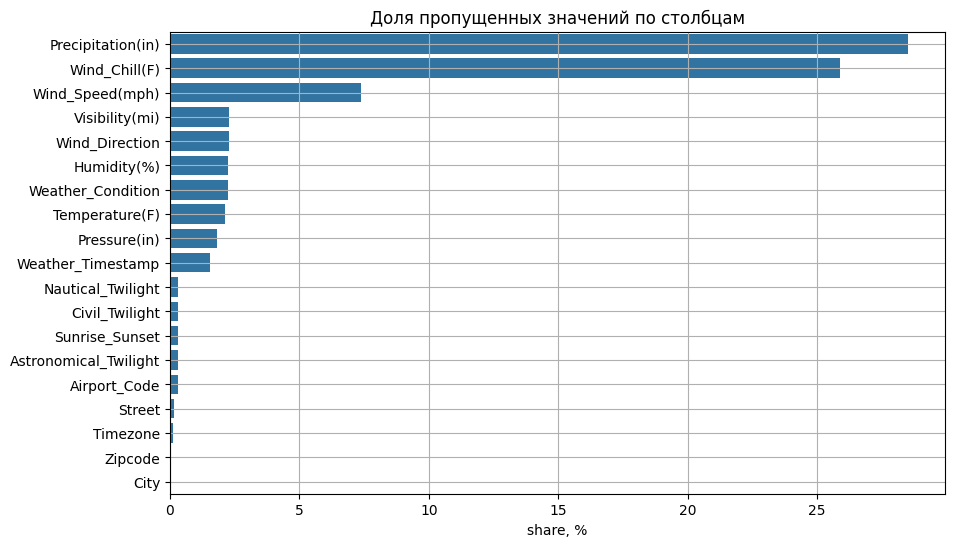
\includegraphics[width=0.88\textwidth]{Content/Images/lab1_missing_values.png}
    \caption{Доля пропущенных значений в признаках набора US Accidents}
    \label{fig:missing-values}
\end{figure}

\vspace{\baselineskip}
\subsection{Анализ целевого признака Severity}
\vspace{\baselineskip}

Признак \texttt{Severity} принимает четыре значения. Распределение записей по классам приведено в таблице~\ref{tab:severity-dist}.

\begin{table}[H]
    \centering
    \caption{Распределение происшествий по признаку Severity}
    \label{tab:severity-dist}
    \small
    \begin{tabular}{|c|r|r|}
        \hline
        \centering Значение Severity & \centering\arraybackslash Количество записей & \centering\arraybackslash Доля, \% \\
        \hline
        1 & 67\,366 & 0,87 \\
        \hline
        2 & 6\,156\,981 & 79,67 \\
        \hline
        3 & 1\,299\,337 & 16,81 \\
        \hline
        4 & 204\,710 & 2,65 \\
        \hline
        Итого & 7\,728\,394 & 100,00 \\
        \hline
    \end{tabular}
\end{table}

Распределение классов существенно несбалансировано: почти 80\,\% записей относятся ко второму классу тяжести. Это обстоятельство необходимо учитывать при построении классификаторов. В частности, простая метрика accuracy может создавать завышенное представление о качестве модели, поэтому в дальнейшем дополнительно используются precision, recall, F1 и AUC ROC.

Для наглядного сравнения частот классов в ноутбуке построена диаграмма распределения признака \texttt{Severity}. Она показывает доминирование второго класса и существенно меньшую представленность первого и четвёртого классов. Это визуально подтверждает необходимость учитывать дисбаланс при обучении классификатора.

\begin{figure}[H]
    \centering
    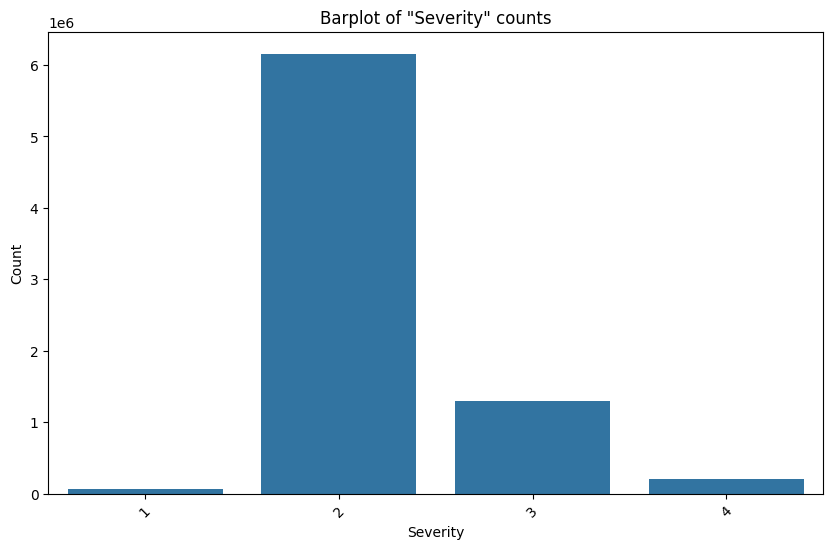
\includegraphics[width=0.78\textwidth]{Content/Images/lab1_severity_distribution.png}
    \caption{Распределение количества происшествий по уровням Severity}
    \label{fig:severity-distribution}
\end{figure}

\vspace{\baselineskip}
\subsection{Выявление и обработка выбросов}
\vspace{\baselineskip}

Для числовых признаков были рассчитаны описательные статистики и квантили. Проверка показала, что распределения длительности происшествия и протяжённости перекрытого участка имеют выраженную асимметрию вправо. Поэтому механическое применение правила Тьюки приводило бы к отнесению значительной доли наблюдений к выбросам.

Для \texttt{Duration\_min} первый квартиль составлял 31,00 мин, медиана -- 74,78 мин, третий квартиль -- 124,90 мин. При этом максимальное значение достигало 2\,812\,939 мин, что соответствует нескольким годам и указывает на ошибку или артефакт исходных данных. Граница Тьюки около 265,8 мин помечала бы как выбросы 731\,676 записей, или 9,47\,\% набора. Для \texttt{Distance(mi)} аналогичный подход также давал чрезмерно большое число подозрительных значений из-за большого количества нулевых и близких к нулю наблюдений.

Распределение длительности до ограничения показано на рисунке~\ref{fig:duration-before}. Оно имеет выраженный правый хвост: небольшое число аномально больших значений существенно увеличивает среднее относительно медианы.

Дополнительную информацию о структуре распределения даёт диаграмма размаха на рисунке~\ref{fig:duration-boxplot}. В отличие от гистограммы, boxplot позволяет одновременно оценить медиану, межквартильный размах и наблюдения за пределами усов. На графике видна сильная асимметрия и большое количество удалённых значений. При этом отдельные точки за усами не следует автоматически считать ошибочными: правило Тьюки помечает статистически необычные наблюдения, но не учитывает предметный смысл длительности происшествия.

\begin{figure}[H]
    \centering
    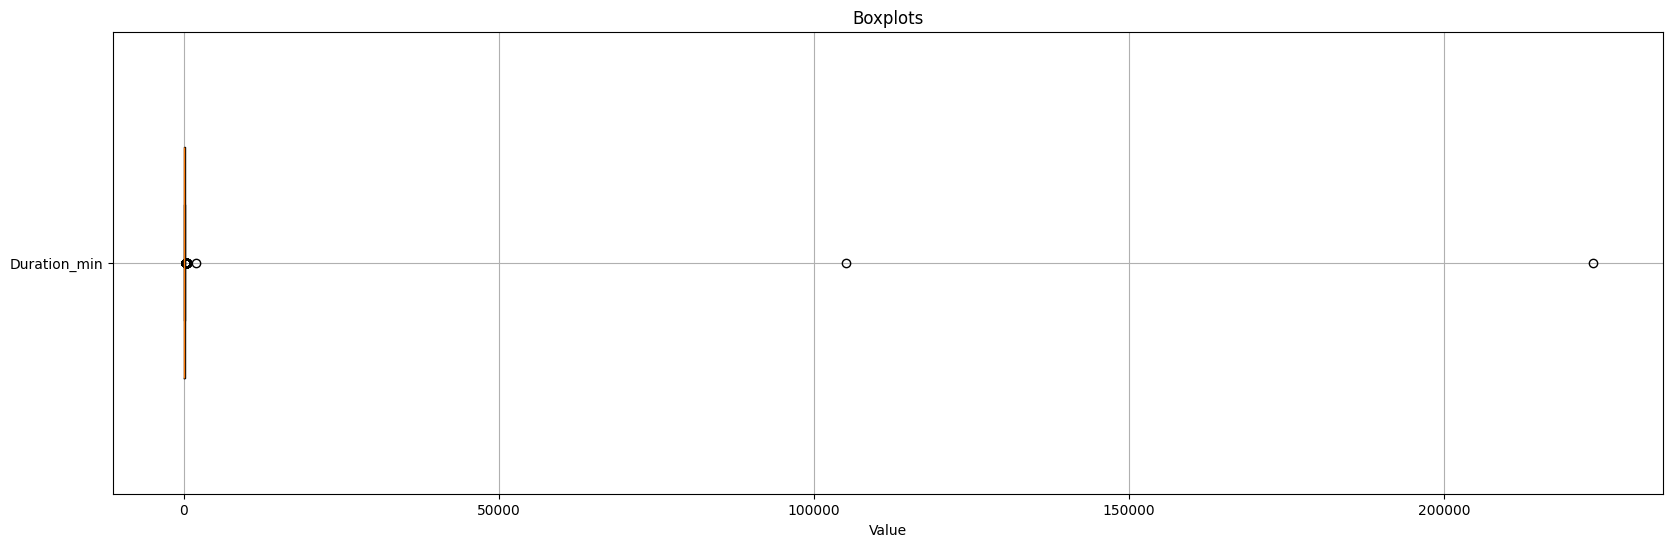
\includegraphics[width=0.88\textwidth]{Content/Images/lab1_boxplot_duration.png}
    \caption{Диаграмма размаха длительности происшествий до винзоризации}
    \label{fig:duration-boxplot}
\end{figure}

\begin{figure}[H]
    \centering
    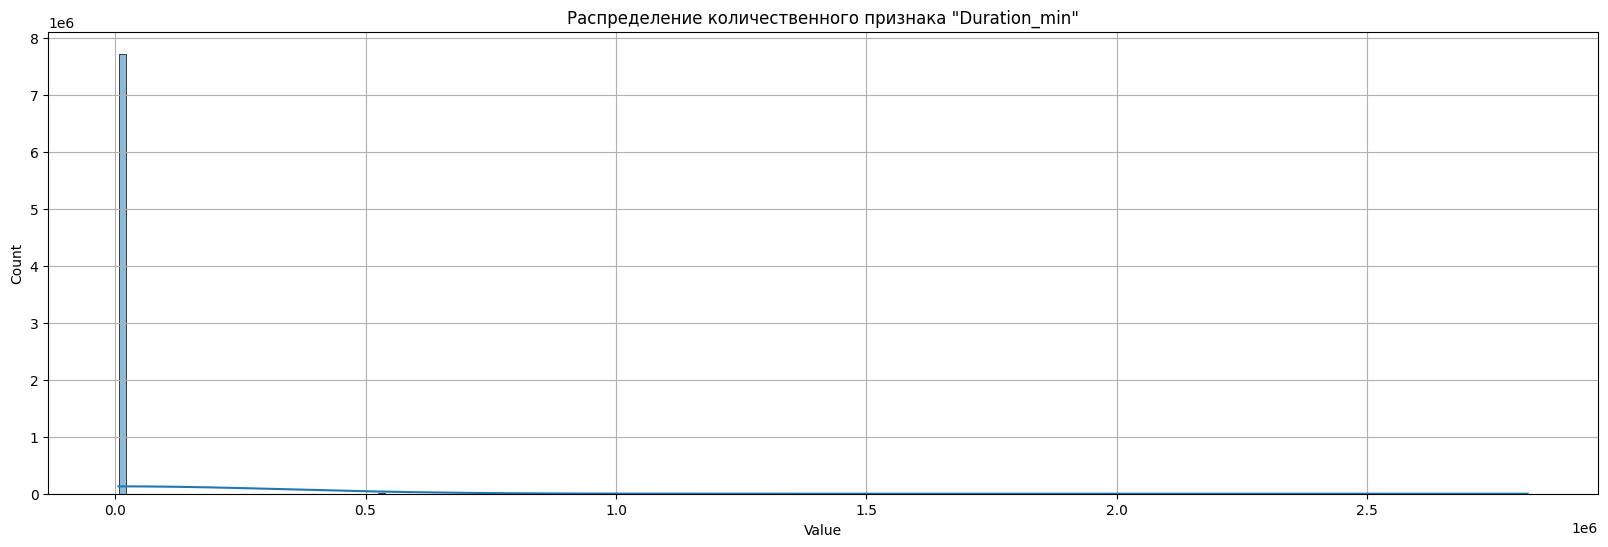
\includegraphics[width=0.82\textwidth]{Content/Images/lab1_duration_distribution.png}
    \caption{Распределение длительности происшествий до винзоризации}
    \label{fig:duration-before}
\end{figure}

Вместо автоматического удаления таких строк были выбраны смысловые верхние границы. Для длительности установлено значение 2880 мин (двое суток), а для протяжённости -- 60 миль. Значения выше соответствующих порогов заменялись выбранными границами. Такая процедура называется винзоризацией. Она позволила ограничить влияние экстремальных значений на статистики, не уменьшая число строк в наборе данных. При пороге длительности 2880 мин затронуто 10\,882 записи (0,141\,\% набора), а при пороге расстояния 60 миль -- 416 записей.

В ноутбуке ограничение длительности выполнялось заменой значений, превышающих 2880 мин, на саму верхнюю границу. Соответствующий фрагмент кода представлен ниже, а распределение после преобразования показано на рисунке~\ref{fig:duration-after}.

\begin{code}
DURATION_CAP = 2880.0
df = df.withColumn(
    "Duration_min",
    when(col("Duration_min") > DURATION_CAP,
         DURATION_CAP).otherwise(col("Duration_min"))
)
\end{code}

После преобразования все значения длительности находятся в диапазоне от исходного минимума до 2880 мин. При этом количество наблюдений сохраняется, а влияние экстремального правого хвоста на последующие вычисления уменьшается.

Для признака \texttt{Distance(mi)} в ноутбуке также построена диаграмма размаха (рисунок~\ref{fig:distance-boxplot}). Её распределение характеризуется концентрацией значений в нижней части шкалы и большим числом точек за верхним усом. Граница Тьюки около 1,15 мили помечает значительную долю наблюдений, поэтому удалять все такие записи было бы некорректно. В исследовании вместо этого использована предметно обоснованная граница 60 миль; ей соответствуют только 416 значений, превышающих порог.

\begin{figure}[H]
    \centering
    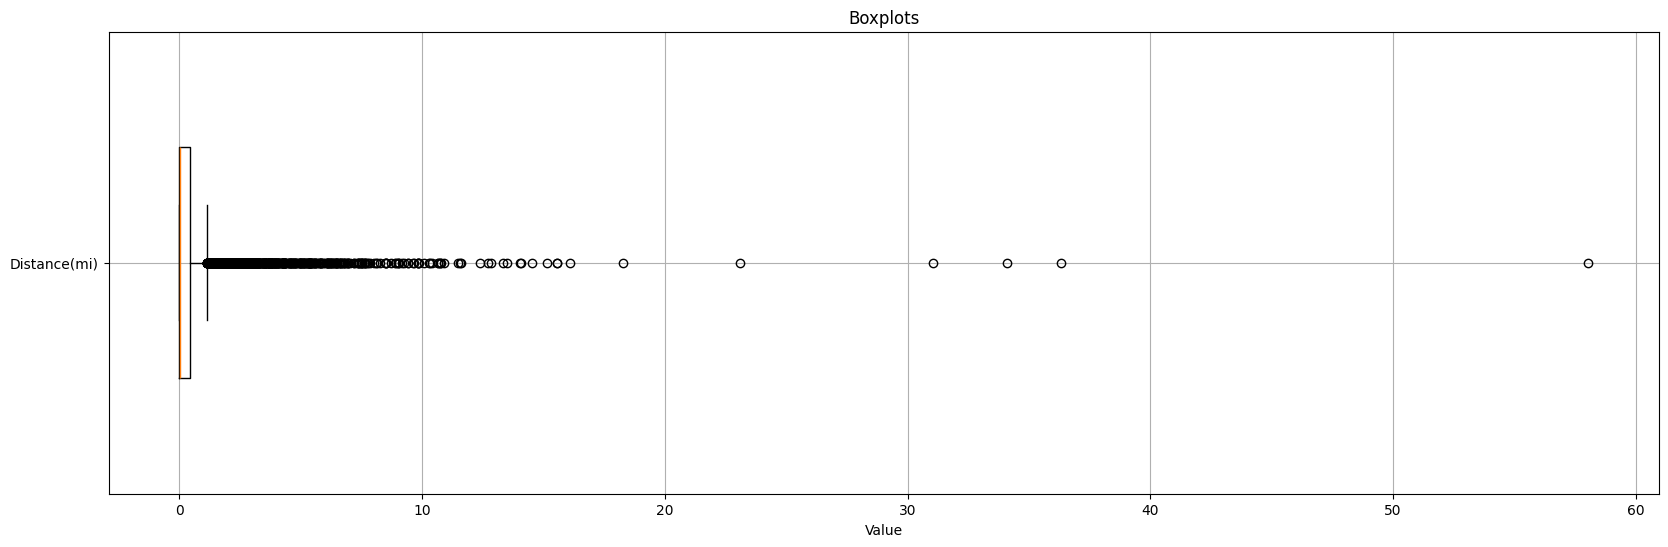
\includegraphics[width=0.88\textwidth]{Content/Images/lab1_boxplot_distance.png}
    \caption{Диаграмма размаха протяжённости участка происшествия}
    \label{fig:distance-boxplot}
\end{figure}

\begin{figure}[H]
    \centering
    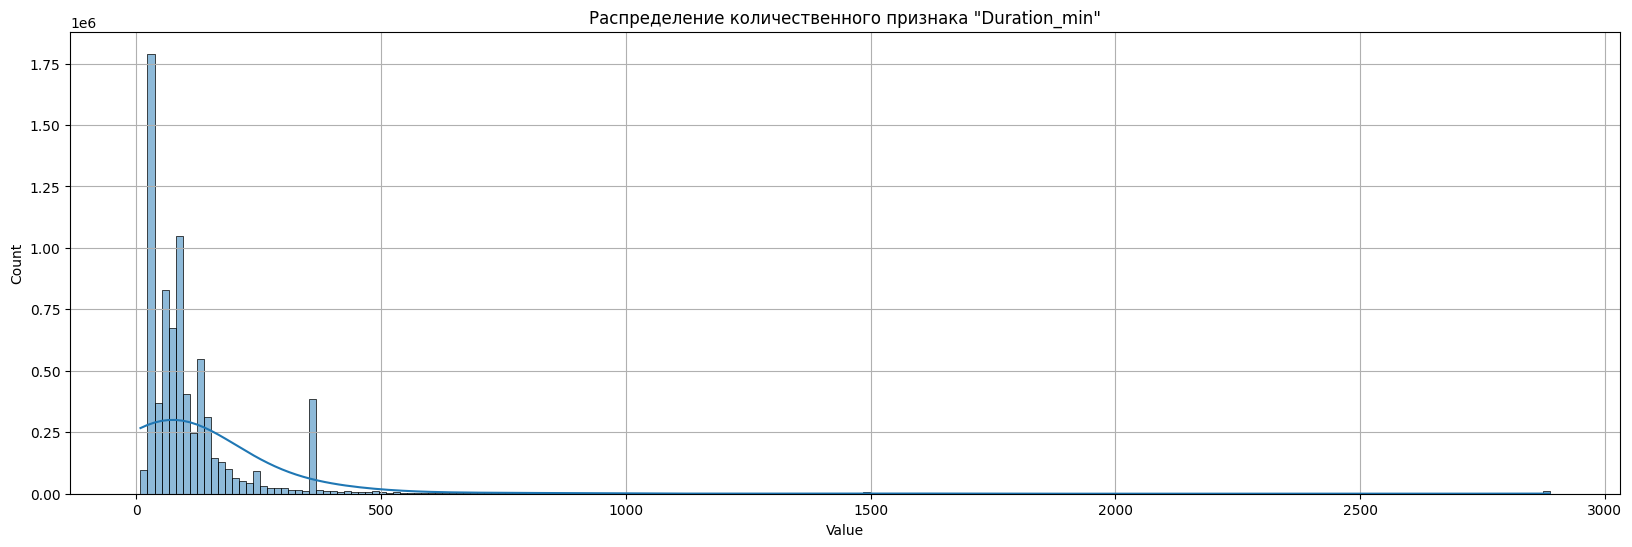
\includegraphics[width=0.82\textwidth]{Content/Images/lab1_duration_capped.png}
    \caption{Распределение длительности после ограничения верхней границы}
    \label{fig:duration-after}
\end{figure}

%\vspace{\baselineskip}
\subsection{Проверка аномальных погодных значений}
\vspace{\baselineskip}

Дополнительно были выявлены значения погодных признаков, выходящие за физически допустимые диапазоны. Например, для скорости ветра встречались значения до 1087 миль в час, для видимости -- до 140 миль, а для атмосферного давления -- до 58,63 дюйма ртутного столба. Подобные значения не соответствуют реальным условиям наблюдения и могут искажать результаты статистического анализа и обучения моделей.

Значения, выходящие за установленные физические границы, заменялись на пропуски. Затем пропуски в числовых погодных признаках заполнялись медианами соответствующих столбцов. Медиана была выбрана вместо среднего арифметического, поскольку распределения ряда погодных показателей асимметричны и содержат экстремальные значения. После выполнения этих операций пропуски в погодных числовых признаках были устранены.


Для дополнительного анализа сезонной изменчивости в ноутбуке построены диаграммы размаха температуры по месяцам (рисунок~\ref{fig:temperature-month-boxplot}). Медианные значения и межквартильные интервалы различаются в зависимости от месяца, что отражает сезонный характер погодного признака. Наличие отдельных значений за пределами усов также показывает, что даже после очистки в данных сохраняется естественная вариативность температуры, которую не следует смешивать с ошибками измерения.

\begin{figure}[H]
    \centering
    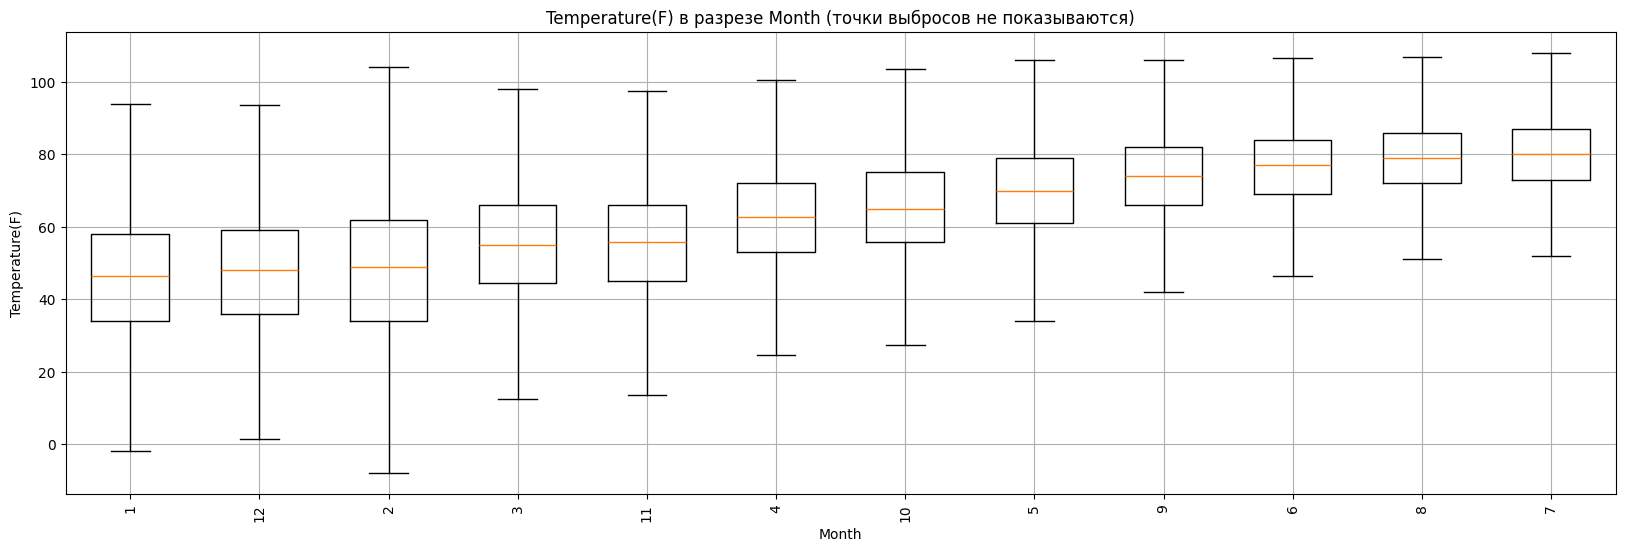
\includegraphics[width=0.88\textwidth]{Content/Images/lab1_temperature_by_month_boxplot.png}
    \caption{Распределение температуры по месяцам года}
    \label{fig:temperature-month-boxplot}
\end{figure}

%\vspace{\baselineskip}
\subsection{Преобразование категориальных и логических признаков}
\vspace{\baselineskip}

В категориальных признаках были обнаружены высокая кардинальность, различные варианты написания одинаковых значений и редкие категории. Например, признак \texttt{Street} содержал 336\,306 различных значений, а \texttt{Zipcode} -- 825\,094. Использование таких признаков без преобразования существенно увеличивало бы размерность пространства признаков. Поэтому \texttt{Street} был исключён, а почтовые индексы приведены к формату из пяти цифр.

В признаке \texttt{Weather\_Condition} редкие категории были объединены в категорию \texttt{Other}. В признаке \texttt{Wind\_Direction} выполнены удаление лишних пробелов, приведение строк к нижнему регистру и объединение полных названий сторон света с их сокращениями. В результате число уровней признака было сокращено до 19, включая значения \texttt{calm}, \texttt{var} и \texttt{unknown}.

Для логических признаков была рассчитана доля значений \texttt{true}. Было установлено, что признаки \texttt{Bump}, \texttt{Roundabout} и \texttt{Turning\_Loop} имеют крайне низкую вариативность. Они были исключены из подготовленного набора, поскольку практически не содержат информации для различения наблюдений.

Дополнительно была исследована связь длительности происшествий с уровнем тяжести. На рисунке~\ref{fig:duration-severity} представлены распределения \texttt{Duration\_min} для различных значений \texttt{Severity}. Различия между группами демонстрируют, что тяжесть события связана с распределением длительности, хотя сама по себе такая связь не означает причинной зависимости.

\begin{figure}[H]
    \centering
    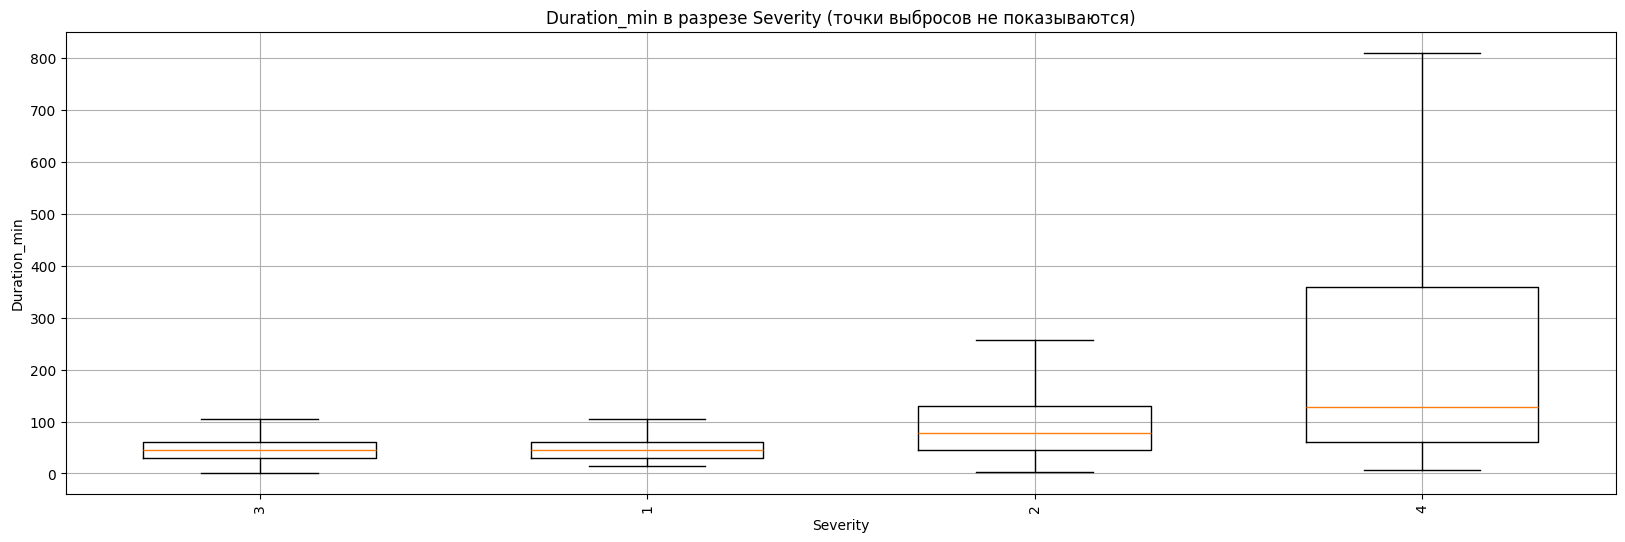
\includegraphics[width=0.88\textwidth]{Content/Images/lab1_duration_by_severity.png}
    \caption{Распределение длительности происшествий в разрезе Severity}
    \label{fig:duration-severity}
\end{figure}

Для оценки линейной зависимости между числовыми характеристиками была построена корреляционная матрица. Её визуализация приведена на рисунке~\ref{fig:correlation-matrix}. Матрица использовалась как инструмент первичного анализа связей и помогла оценить, насколько отдельные количественные признаки могут объяснять целевые переменные последующего моделирования.

\begin{figure}[H]
    \centering
    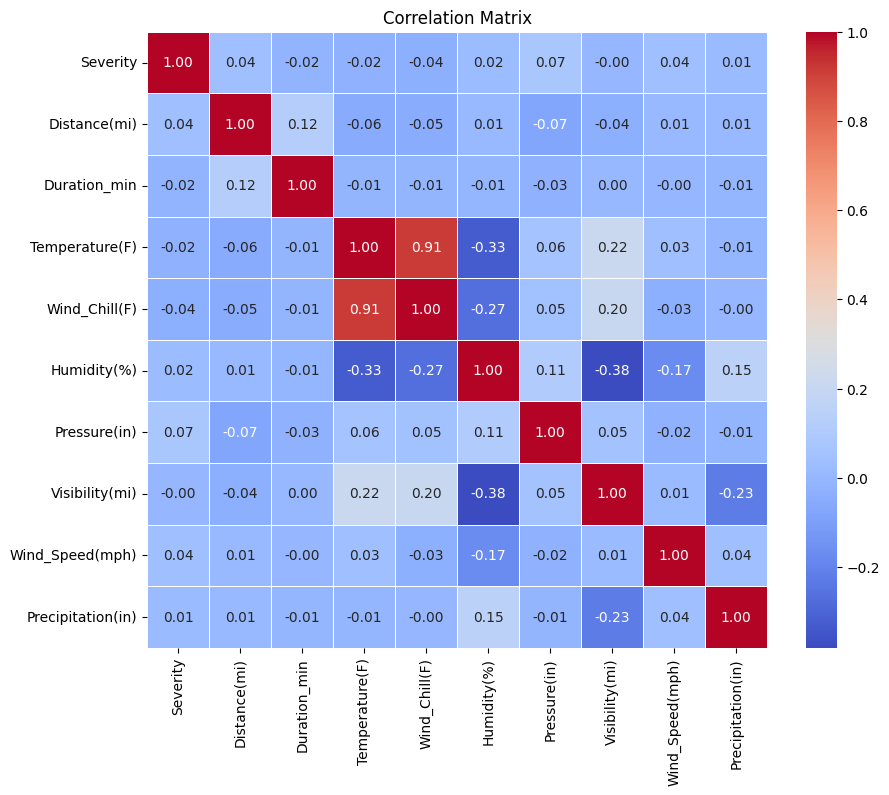
\includegraphics[width=0.88\textwidth]{Content/Images/lab1_correlation_matrix.png}
    \caption{Корреляционная матрица числовых признаков набора US Accidents}
    \label{fig:correlation-matrix}
\end{figure}

Из временной метки начала происшествия были дополнительно извлечены месяц, день недели и час. Эти признаки позволяют учитывать временные закономерности возникновения аварий без непосредственного использования исходной временной метки в моделях. Диаграмма на рисунке~\ref{fig:accidents-by-hour} показывает изменение числа зарегистрированных происшествий в течение суток. Видно, что интенсивность регистрации меняется в зависимости от часа, поэтому временной признак может содержать полезную информацию для последующего моделирования.

\begin{figure}[H]
    \centering
    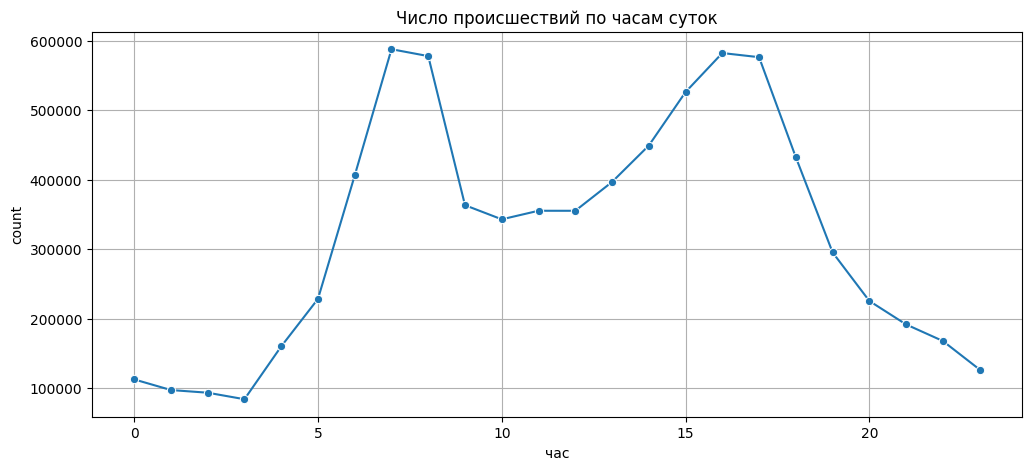
\includegraphics[width=0.88\textwidth]{Content/Images/lab1_accidents_by_hour.png}
    \caption{Количество зарегистрированных происшествий в зависимости от часа суток}
    \label{fig:accidents-by-hour}
\end{figure}

%\vspace{\baselineskip}
\section{Выводы}
\vspace{\baselineskip}

В первой главе рассмотрен набор данных US Accidents и выполнена его первичная подготовка средствами Apache Spark. Исходный файл объёмом около 2,84 ГиБ содержит 7\,728\,394 записи и 46 столбцов. После отбора признаков, преобразования типов и вычисления длительности происшествия была сформирована таблица из 40 полей, сохранённая в формате Apache Iceberg. Контрольное количество строк совпало с количеством записей исходного файла.

В ходе разведочного анализа выявлены пропуски в погодных характеристиках, несбалансированность целевого признака \texttt{Severity}, экстремальные значения длительности и расстояния, а также аномальные погодные показатели. Для обработки данных использовались заполнение пропусков, проверка физических диапазонов, винзоризация числовых признаков, объединение редких категорий и исключение признаков с высокой кардинальностью или низкой вариативностью.

Полученная таблица подготовлена для последующего машинного обучения. При этом выявленные особенности данных -- в частности, несбалансированность классов и слабая связь ряда числовых признаков с длительностью происшествия -- учитываются при выборе моделей и метрик качества во второй главе.